\documentclass[tikz,border=10pt]{standalone}
% Only TikZ libraries are needed here (none beyond the core).
\begin{document}
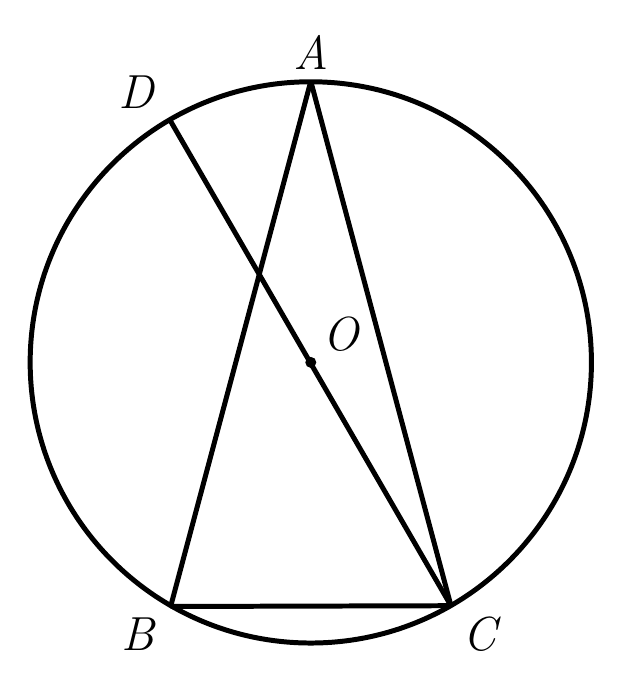
\begin{tikzpicture}[line width=1.8pt, line join=round]
  % Coordinates: O at origin; s = 0.022663 cm/px (STYLE METRICS scale)
  \coordinate (O) at (0,0);
  \coordinate (A) at (0,3.57);
  \coordinate (B) at (-1.78,-3.10);
  \coordinate (C) at (1.78,-3.09);
  \coordinate (D) at (-1.79,3.08);

  % Circle, radius 157.27 px
  \draw (O) circle[radius=3.564];

  % Chords and diameter DC (passes through O)
  \draw (A) -- (B);
  \draw (A) -- (C);
  \draw (B) -- (C);
  \draw (D) -- (C);

  % Centre dot
  \fill (O) circle[radius=0.07];

  % Labels, font calibrated to STYLE METRICS
  \node[above] at (A) {\fontsize{19}{22.8}\selectfont $\mathit{A}$};
  \node[below left] at (B) {\fontsize{19}{22.8}\selectfont $\mathit{B}$};
  \node[below right] at (C) {\fontsize{19}{22.8}\selectfont $\mathit{C}$};
  \node[above left] at (D) {\fontsize{19}{22.8}\selectfont $\mathit{D}$};
  \node[above right] at (O) {\fontsize{19}{22.8}\selectfont $\mathit{O}$};
\end{tikzpicture}
\end{document}